\subsection{New completed breadth-cohort loss curves}
\label{app:breadth-loss-updates}
Every displayed cohort contains five completed full-budget methods. Learning rates are selected on validation only after both predeclared rates have completed for every method; otherwise a completed common-rate cohort is labeled fixed-rate. Each curve is traced to its complete log in the accompanying audit.
\begin{figure}[!htbp]
\centering
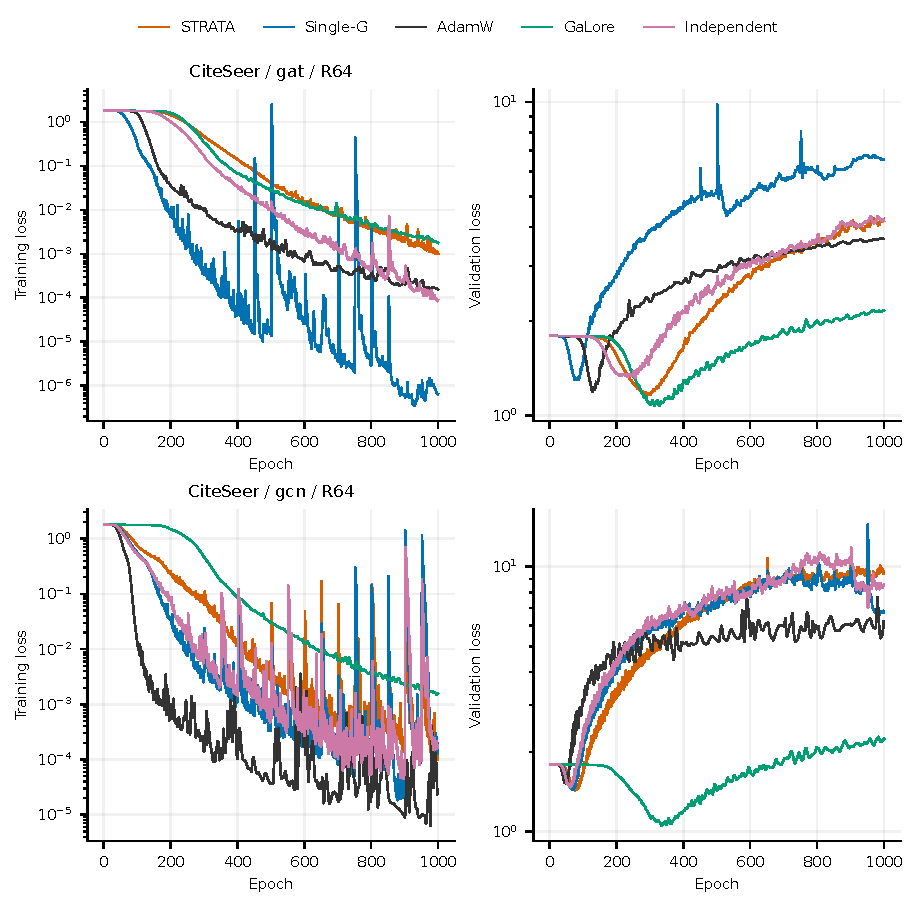
\includegraphics[width=.98\linewidth]{figures/fig_breadth_complete_00.pdf}
\caption{\textbf{Completed breadth-cohort training and validation losses.} CiteSeer/gat: two-rate validation selection; CiteSeer/gcn: two-rate validation selection. Left: training; right: validation. Raw complete trajectories, seed 42. No smoothing or extrapolation.}
\end{figure}
\begin{figure}[!htbp]
\centering
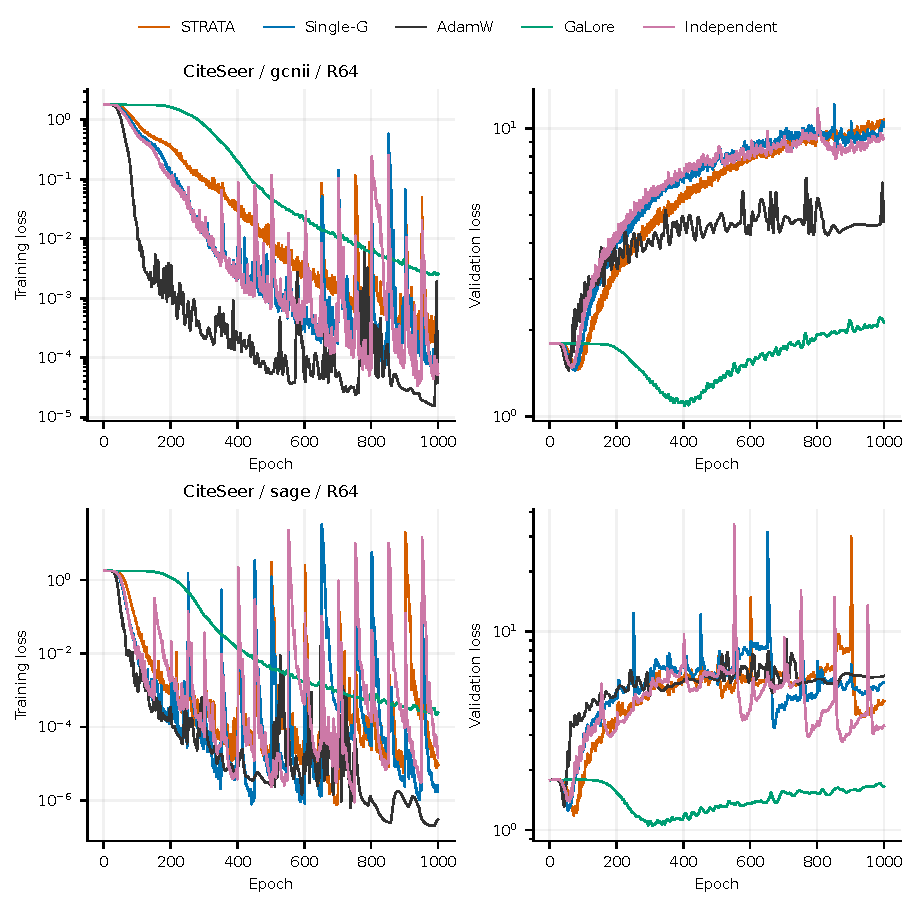
\includegraphics[width=.98\linewidth]{figures/fig_breadth_complete_01.pdf}
\caption{\textbf{Completed breadth-cohort training and validation losses.} CiteSeer/gcnii: two-rate validation selection; CiteSeer/sage: two-rate validation selection. Left: training; right: validation. Raw complete trajectories, seed 42. No smoothing or extrapolation.}
\end{figure}
\begin{figure}[!htbp]
\centering
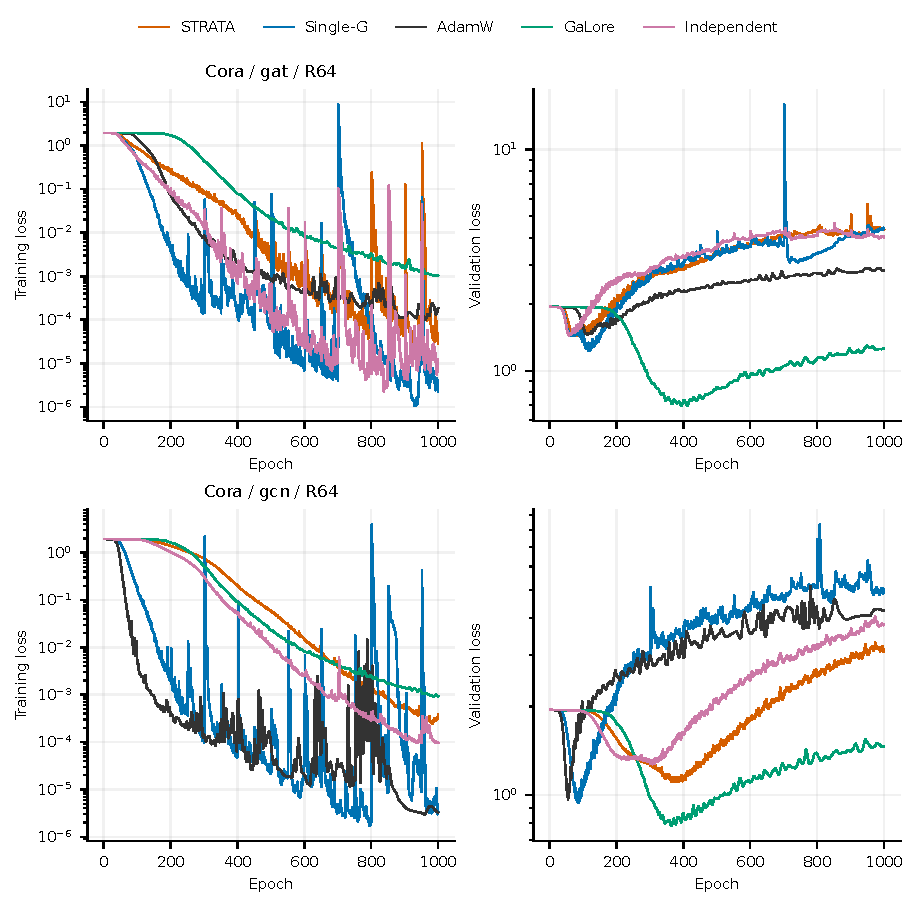
\includegraphics[width=.98\linewidth]{figures/fig_breadth_complete_02.pdf}
\caption{\textbf{Completed breadth-cohort training and validation losses.} Cora/gat: two-rate validation selection; Cora/gcn: two-rate validation selection. Left: training; right: validation. Raw complete trajectories, seed 42. No smoothing or extrapolation.}
\end{figure}
\begin{figure}[!htbp]
\centering
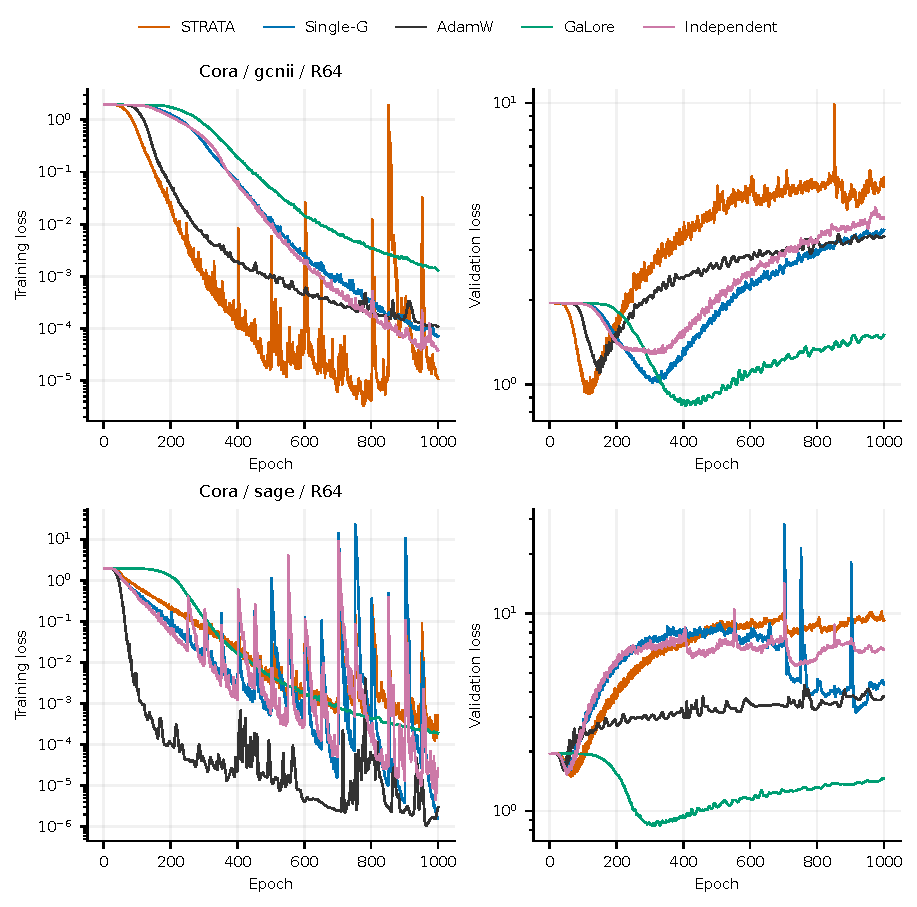
\includegraphics[width=.98\linewidth]{figures/fig_breadth_complete_03.pdf}
\caption{\textbf{Completed breadth-cohort training and validation losses.} Cora/gcnii: two-rate validation selection; Cora/sage: two-rate validation selection. Left: training; right: validation. Raw complete trajectories, seed 42. No smoothing or extrapolation.}
\end{figure}
\begin{figure}[!htbp]
\centering
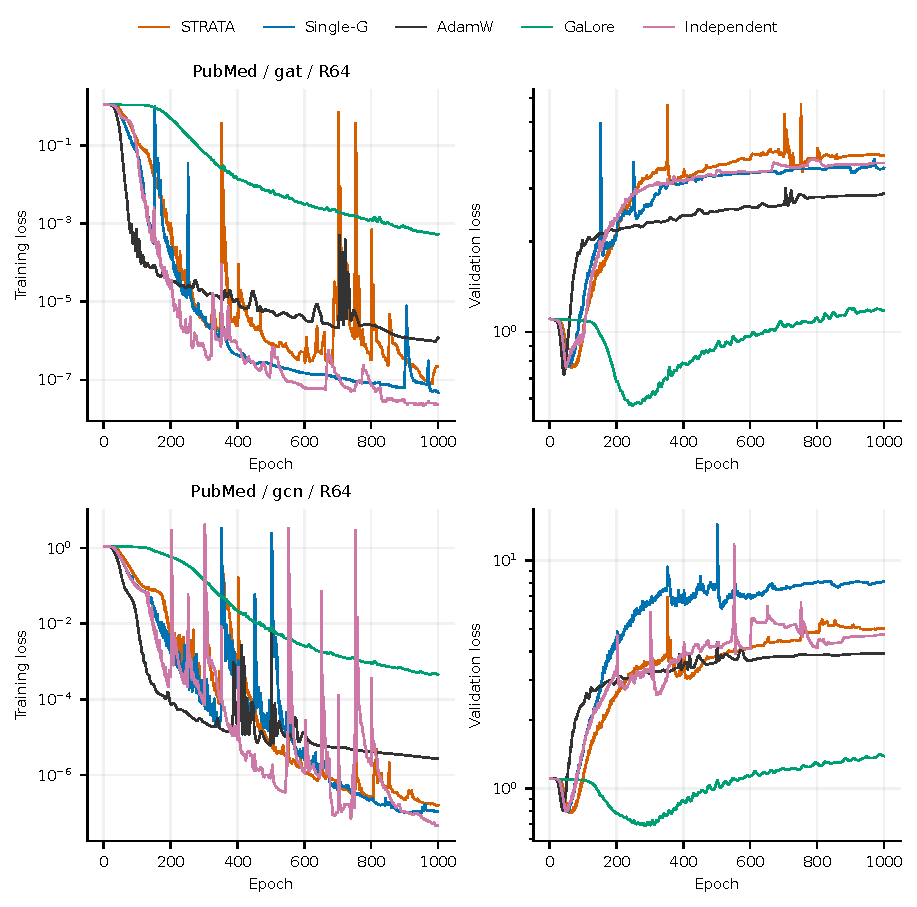
\includegraphics[width=.98\linewidth]{figures/fig_breadth_complete_04.pdf}
\caption{\textbf{Completed breadth-cohort training and validation losses.} PubMed/gat: two-rate validation selection; PubMed/gcn: two-rate validation selection. Left: training; right: validation. Raw complete trajectories, seed 42. No smoothing or extrapolation.}
\end{figure}
\begin{figure}[!htbp]
\centering
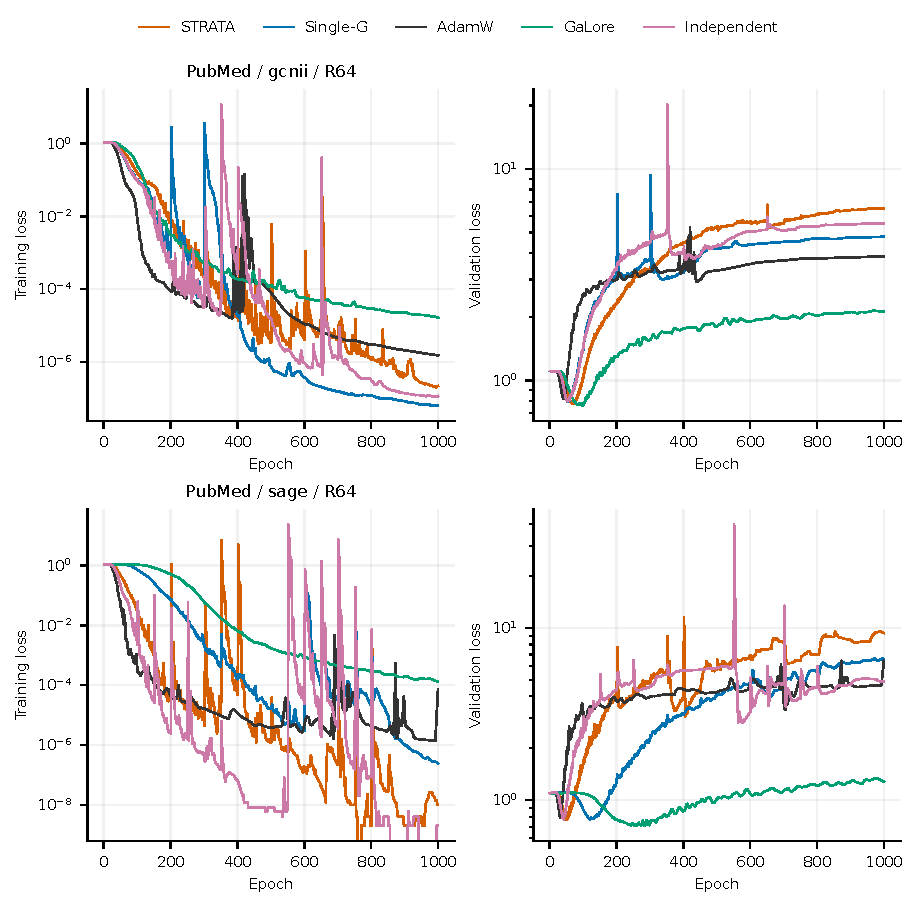
\includegraphics[width=.98\linewidth]{figures/fig_breadth_complete_05.pdf}
\caption{\textbf{Completed breadth-cohort training and validation losses.} PubMed/gcnii: two-rate validation selection; PubMed/sage: two-rate validation selection. Left: training; right: validation. Raw complete trajectories, seed 42. No smoothing or extrapolation.}
\end{figure}
\begin{figure}[!htbp]
\centering
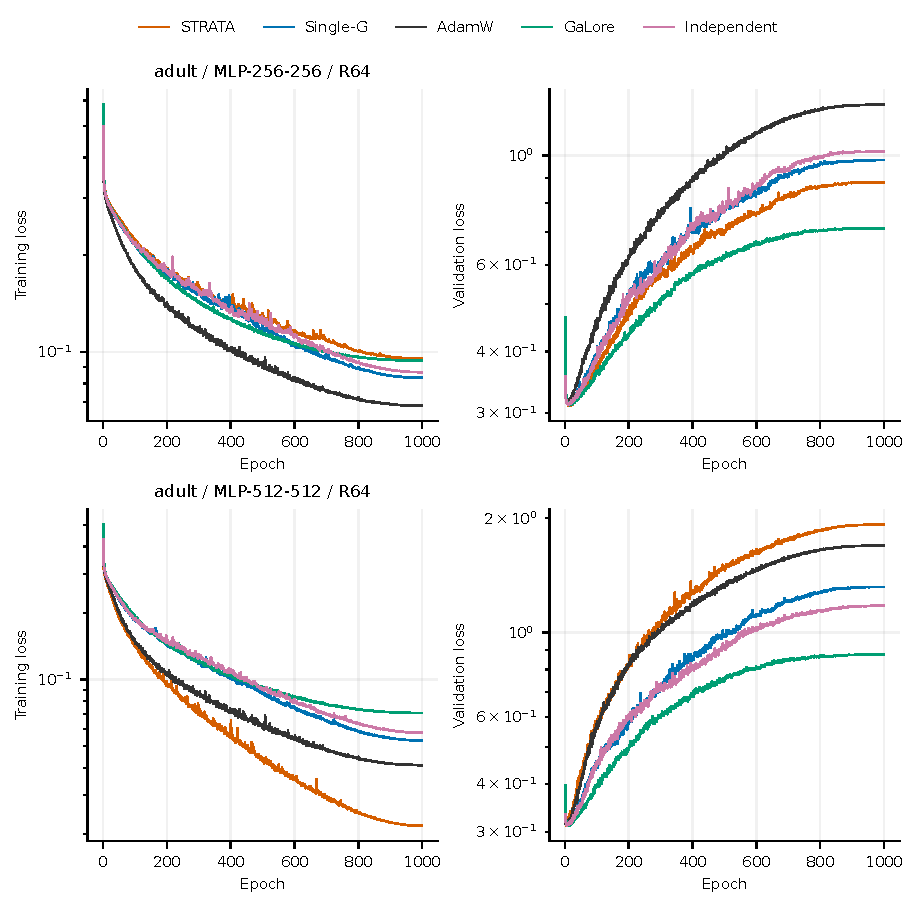
\includegraphics[width=.98\linewidth]{figures/fig_breadth_complete_06.pdf}
\caption{\textbf{Completed breadth-cohort training and validation losses.} adult/MLP-256-256: two-rate validation selection; adult/MLP-512-512: two-rate validation selection. Left: training; right: validation. Raw complete trajectories, seed 42. No smoothing or extrapolation.}
\end{figure}
\begin{figure}[!htbp]
\centering
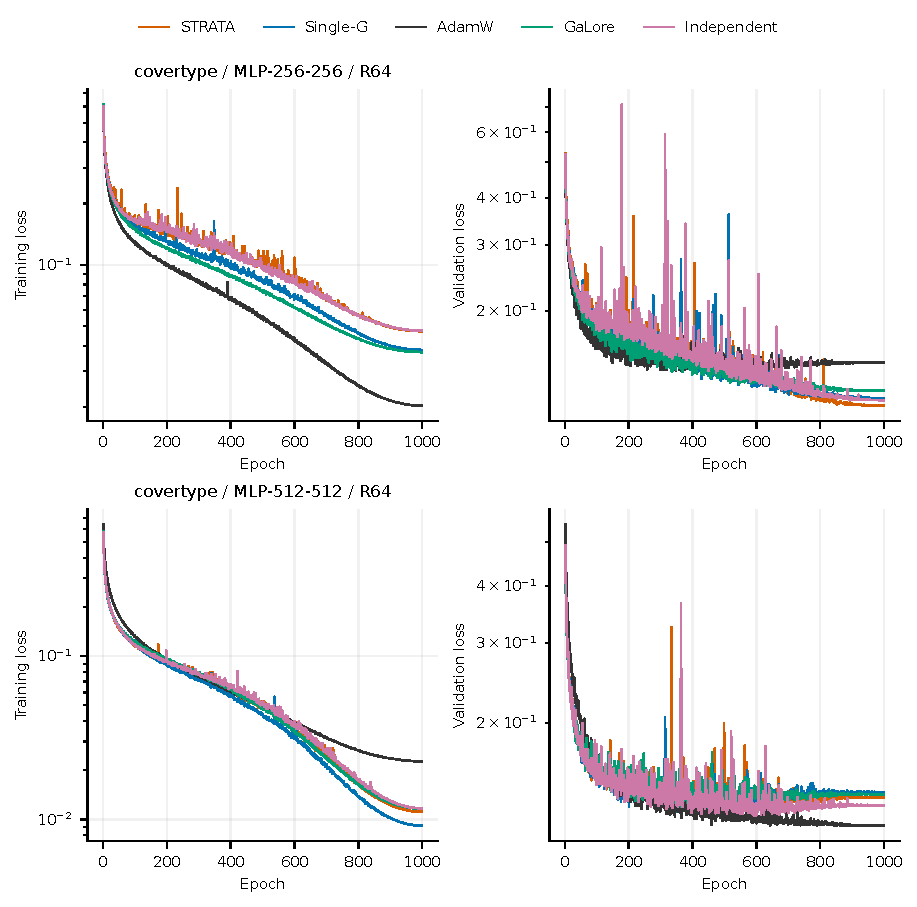
\includegraphics[width=.98\linewidth]{figures/fig_breadth_complete_07.pdf}
\caption{\textbf{Completed breadth-cohort training and validation losses.} covertype/MLP-256-256: two-rate validation selection; covertype/MLP-512-512: two-rate validation selection. Left: training; right: validation. Raw complete trajectories, seed 42. No smoothing or extrapolation.}
\end{figure}
\begin{figure}[!htbp]
\centering
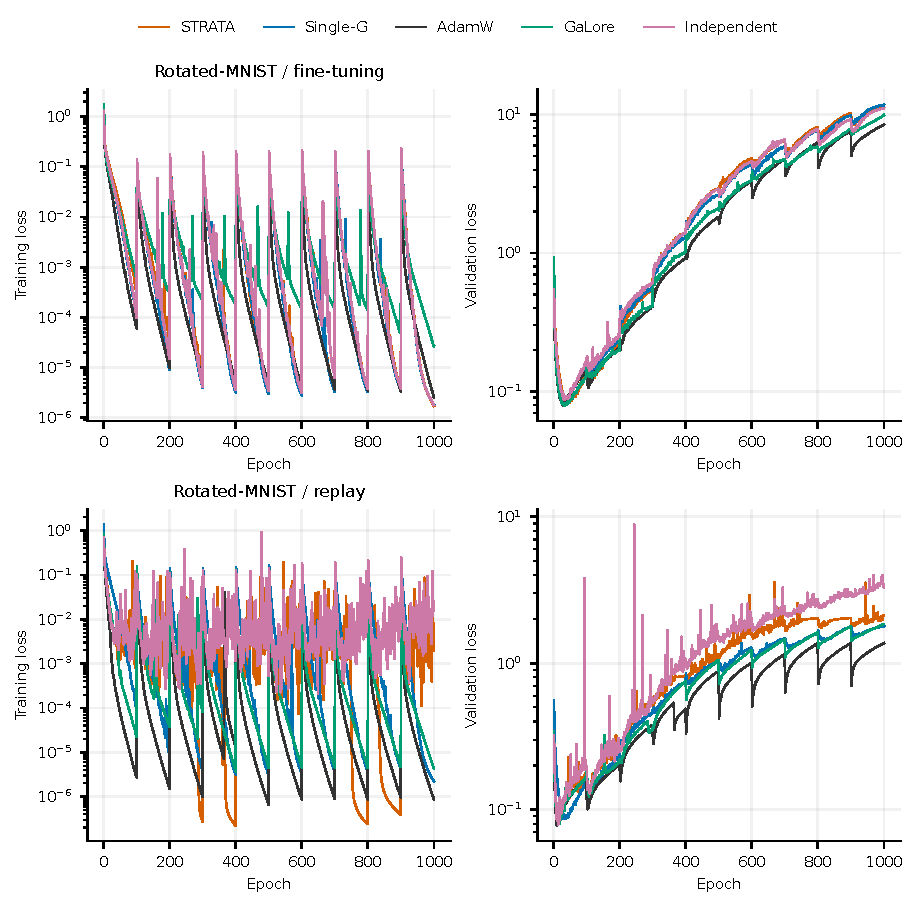
\includegraphics[width=.98\linewidth]{figures/fig_breadth_complete_08.pdf}
\caption{\textbf{Completed breadth-cohort training and validation losses.} rotated\_mnist\_cl/MLP-256-256/finetune: two-rate validation selection; rotated\_mnist\_cl/MLP-256-256/replay: two-rate validation selection. Left: training; right: validation. Raw complete trajectories, seed 42. Continual validation averages seen tasks, so its evaluation distribution changes at task boundaries. No smoothing or extrapolation.}
\end{figure}
\begin{figure}[!htbp]
\centering
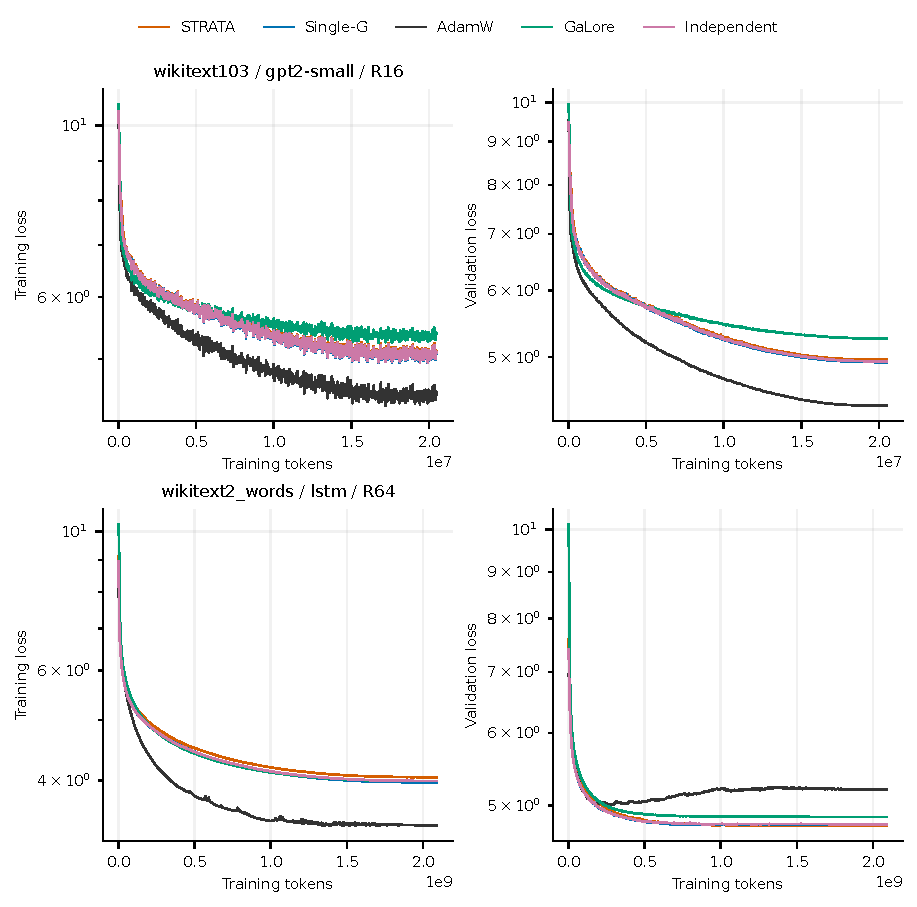
\includegraphics[width=.98\linewidth]{figures/fig_breadth_complete_09.pdf}
\caption{\textbf{Completed breadth-cohort training and validation losses.} wikitext103/gpt2-small: two-rate validation selection; wikitext2\_words/lstm: fixed rate 0.0003; search incomplete. Left: training; right: validation. Raw complete trajectories, seed 42. No smoothing or extrapolation.}
\end{figure}
\begin{figure}[!htbp]
\centering
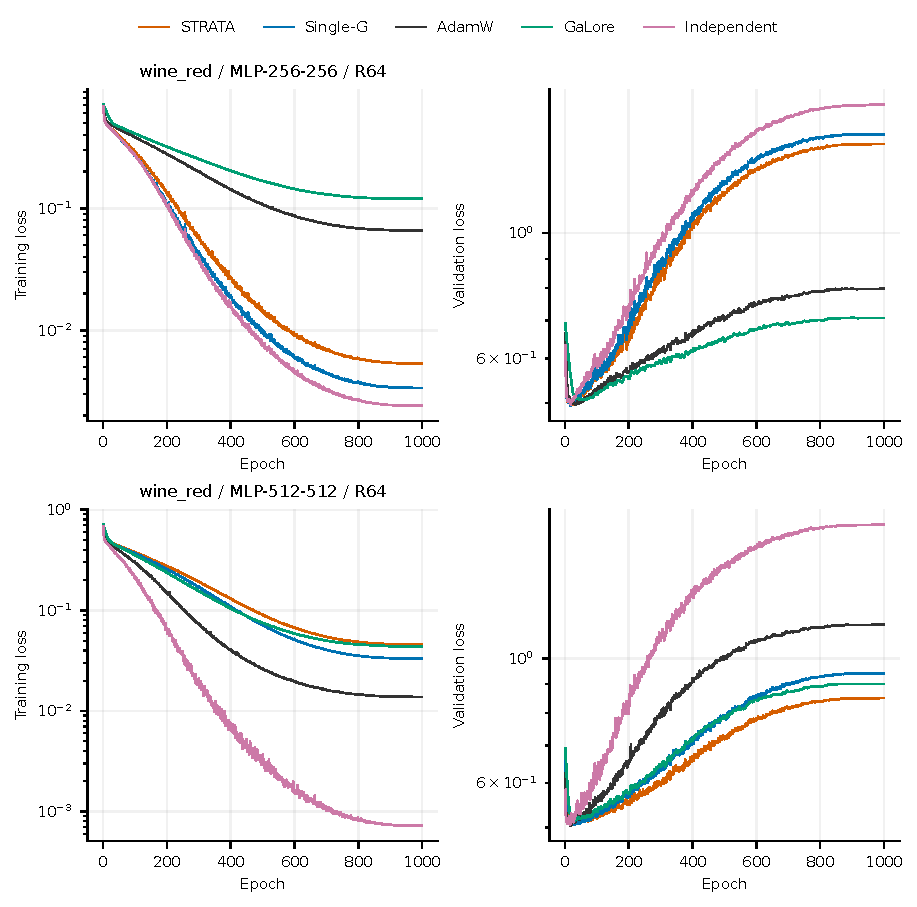
\includegraphics[width=.98\linewidth]{figures/fig_breadth_complete_10.pdf}
\caption{\textbf{Completed breadth-cohort training and validation losses.} wine\_red/MLP-256-256: two-rate validation selection; wine\_red/MLP-512-512: two-rate validation selection. Left: training; right: validation. Raw complete trajectories, seed 42. No smoothing or extrapolation.}
\end{figure}
\begin{figure}[!htbp]
\centering
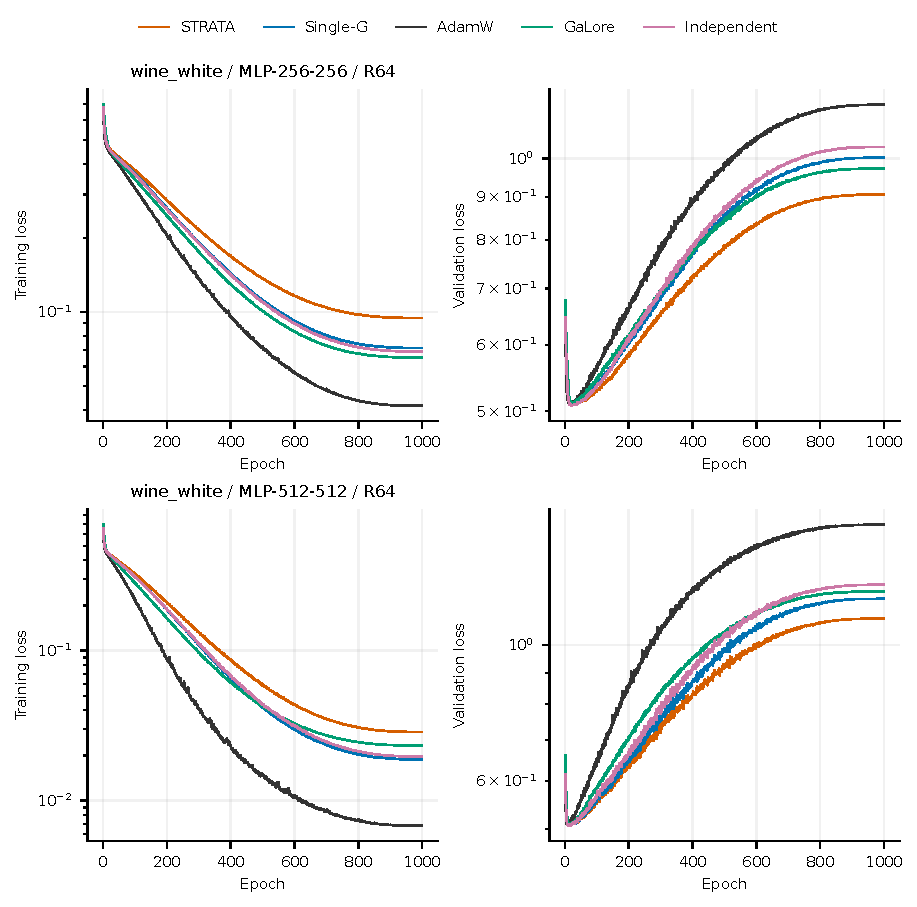
\includegraphics[width=.98\linewidth]{figures/fig_breadth_complete_11.pdf}
\caption{\textbf{Completed breadth-cohort training and validation losses.} wine\_white/MLP-256-256: two-rate validation selection; wine\_white/MLP-512-512: two-rate validation selection. Left: training; right: validation. Raw complete trajectories, seed 42. No smoothing or extrapolation.}
\end{figure}
